

\tikzset{every picture/.style={line width=0.75pt}} %set default line width to 0.75pt        

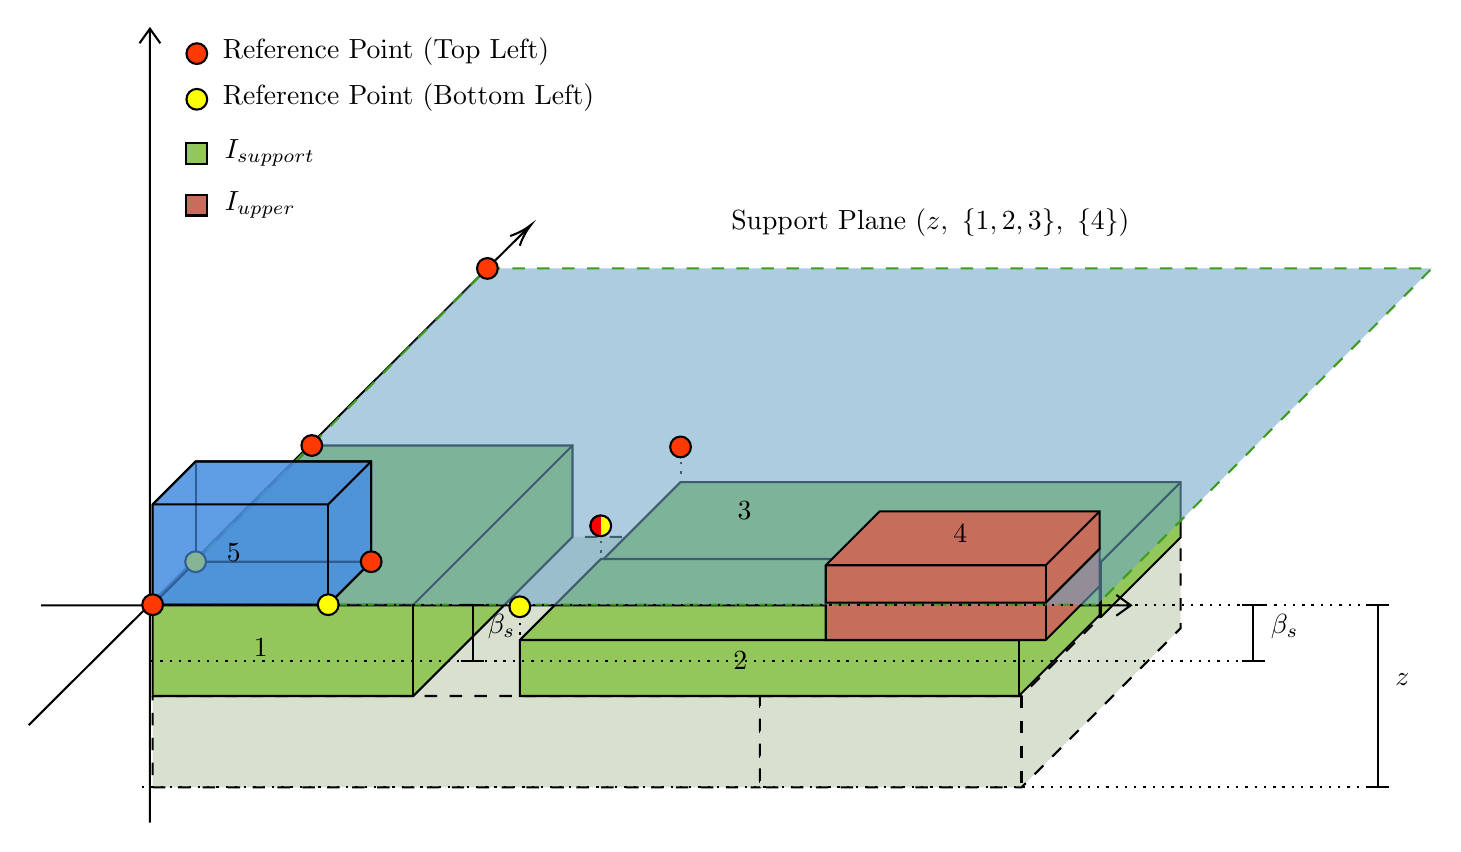
\begin{tikzpicture}[x=0.75pt,y=0.75pt,yscale=-1,xscale=1]
%uncomment if require: \path (0,533); %set diagram left start at 0, and has height of 533

%Shape: Cube [id:dp7106500856615827] 
\draw  [fill={rgb, 255:red, 216; green, 224; blue, 207 }  ,fill opacity=1 ][dash pattern={on 4.5pt off 4.5pt}] (75.7,462.5) -- (152.4,385.81) -- (445,385.81) -- (445,429.81) -- (368.31,506.5) -- (75.7,506.5) -- cycle ; \draw  [dash pattern={on 4.5pt off 4.5pt}] (445,385.81) -- (368.31,462.5) -- (75.7,462.5) ; \draw  [dash pattern={on 4.5pt off 4.5pt}] (368.31,462.5) -- (368.31,506.5) ;
%Straight Lines [id:da8316956251676535] 
\draw  [dash pattern={on 0.84pt off 2.51pt}]  (291.62,397.89) -- (291.62,380.5) ;
%Straight Lines [id:da38384433092333237] 
\draw  [dash pattern={on 0.84pt off 2.51pt}]  (330.05,359.89) -- (330.05,342.5) ;
%Shape: Cube [id:dp47709739603214574] 
\draw  [fill={rgb, 255:red, 216; green, 224; blue, 207 }  ,fill opacity=1 ][dash pattern={on 4.5pt off 4.5pt}] (368.31,462.5) -- (445,385.81) -- (571,385.81) -- (571,429.81) -- (494.31,506.5) -- (368.31,506.5) -- cycle ; \draw  [dash pattern={on 4.5pt off 4.5pt}] (571,385.81) -- (494.31,462.5) -- (368.31,462.5) ; \draw  [dash pattern={on 4.5pt off 4.5pt}] (494.31,462.5) -- (494.31,506.5) ;
%Shape: Cube [id:dp7977002200403227] 
\draw  [fill={rgb, 255:red, 147; green, 198; blue, 91 }  ,fill opacity=1 ] (75.7,418.5) -- (152.4,341.81) -- (278,341.81) -- (278,385.81) -- (201.31,462.5) -- (75.7,462.5) -- cycle ; \draw   (278,341.81) -- (201.31,418.5) -- (75.7,418.5) ; \draw   (201.31,418.5) -- (201.31,462.5) ;
%Shape: Cube [id:dp7121611670665484] 
\draw  [fill={rgb, 255:red, 147; green, 198; blue, 91 }  ,fill opacity=1 ] (291.62,397.89) -- (330.05,359.46) -- (571,359.46) -- (571,386.06) -- (532.56,424.5) -- (291.62,424.5) -- cycle ; \draw   (571,359.46) -- (532.56,397.89) -- (291.62,397.89) ; \draw   (532.56,397.89) -- (532.56,424.5) ;
%Shape: Cube [id:dp604763542929154] 
\draw  [fill={rgb, 255:red, 147; green, 198; blue, 91 }  ,fill opacity=1 ] (252.62,435.5) -- (291.62,396.5) -- (532,396.5) -- (532,423.5) -- (493,462.5) -- (252.62,462.5) -- cycle ; \draw   (532,396.5) -- (493,435.5) -- (252.62,435.5) ; \draw   (493,435.5) -- (493,462.5) ;
%Shape: Axis 2D [id:dp786981943451631] 
\draw  (22,418.81) -- (547,418.81)(74.4,141) -- (74.4,523.5) (540,413.81) -- (547,418.81) -- (540,423.81) (69.4,148) -- (74.4,141) -- (79.4,148)  ;
%Straight Lines [id:da31524103851047525] 
\draw    (16,476.5) -- (256.58,236.91) ;
\draw [shift={(258,235.5)}, rotate = 135.12] [color={rgb, 255:red, 0; green, 0; blue, 0 }  ][line width=0.75]    (10.93,-3.29) .. controls (6.95,-1.4) and (3.31,-0.3) .. (0,0) .. controls (3.31,0.3) and (6.95,1.4) .. (10.93,3.29)   ;
%Shape: Cube [id:dp6424617162036526] 
\draw  [fill={rgb, 255:red, 198; green, 110; blue, 91 }  ,fill opacity=1 ] (400,417.5) -- (426,391.5) -- (532,391.5) -- (532,409.5) -- (506,435.5) -- (400,435.5) -- cycle ; \draw   (532,391.5) -- (506,417.5) -- (400,417.5) ; \draw   (506,417.5) -- (506,435.5) ;
%Shape: Parallelogram [id:dp3639839698249763] 
\draw  [color={rgb, 255:red, 62; green, 156; blue, 30 }  ,draw opacity=1 ][fill={rgb, 255:red, 110; green, 165; blue, 200 }  ,fill opacity=0.57 ][dash pattern={on 4.5pt off 4.5pt}] (237,256.5) -- (692,256.5) -- (530.7,418.5) -- (75.7,418.5) -- cycle ;
%Shape: Cube [id:dp46874066075395426] 
\draw  [fill={rgb, 255:red, 198; green, 110; blue, 91 }  ,fill opacity=1 ] (400,399.5) -- (426,373.5) -- (532,373.5) -- (532,391.5) -- (506,417.5) -- (400,417.5) -- cycle ; \draw   (532,373.5) -- (506,399.5) -- (400,399.5) ; \draw   (506,399.5) -- (506,417.5) ;
%Straight Lines [id:da11997650250706615] 
\draw    (665.96,418.5) -- (665.96,506.5) ;
\draw [shift={(665.96,506.5)}, rotate = 270] [color={rgb, 255:red, 0; green, 0; blue, 0 }  ][line width=0.75]    (0,5.59) -- (0,-5.59)   ;
\draw [shift={(665.96,418.5)}, rotate = 270] [color={rgb, 255:red, 0; green, 0; blue, 0 }  ][line width=0.75]    (0,5.59) -- (0,-5.59)   ;
%Straight Lines [id:da7479086158615895] 
\draw  [dash pattern={on 0.84pt off 2.51pt}]  (75.7,418.5) -- (671,418.5) ;
%Straight Lines [id:da00936893511639092] 
\draw  [dash pattern={on 0.84pt off 2.51pt}]  (70.66,506.5) -- (665.96,506.5) ;
%Straight Lines [id:da2603505755036556] 
\draw  [dash pattern={on 0.84pt off 2.51pt}]  (75,445.5) -- (606,445.5) ;
%Straight Lines [id:da21695403696781168] 
\draw    (606,418.5) -- (606,445.5) ;
\draw [shift={(606,445.5)}, rotate = 270] [color={rgb, 255:red, 0; green, 0; blue, 0 }  ][line width=0.75]    (0,5.59) -- (0,-5.59)   ;
\draw [shift={(606,418.5)}, rotate = 270] [color={rgb, 255:red, 0; green, 0; blue, 0 }  ][line width=0.75]    (0,5.59) -- (0,-5.59)   ;
%Straight Lines [id:da17628222853988207] 
\draw    (230,418.5) -- (230,445.5) ;
\draw [shift={(230,445.5)}, rotate = 270] [color={rgb, 255:red, 0; green, 0; blue, 0 }  ][line width=0.75]    (0,5.59) -- (0,-5.59)   ;
\draw [shift={(230,418.5)}, rotate = 270] [color={rgb, 255:red, 0; green, 0; blue, 0 }  ][line width=0.75]    (0,5.59) -- (0,-5.59)   ;
%Shape: Cube [id:dp458320338188952] 
\draw  [fill={rgb, 255:red, 74; green, 144; blue, 226 }  ,fill opacity=0.66 ] (181,397.8) -- (160.3,418.5) -- (75.7,418.5) -- (75.7,370.2) -- (96.4,349.5) -- (181,349.5) -- cycle ; \draw   (75.7,418.5) -- (96.4,397.8) -- (181,397.8) ; \draw   (96.4,397.8) -- (96.4,349.5) ;
%Shape: Circle [id:dp9728798663710179] 
\draw  [fill={rgb, 255:red, 252; green, 255; blue, 4 }  ,fill opacity=1 ] (92,175) .. controls (92,172.24) and (94.24,170) .. (97,170) .. controls (99.76,170) and (102,172.24) .. (102,175) .. controls (102,177.76) and (99.76,180) .. (97,180) .. controls (94.24,180) and (92,177.76) .. (92,175) -- cycle ;
%Shape: Circle [id:dp41733873180988235] 
\draw  [fill={rgb, 255:red, 252; green, 255; blue, 4 }  ,fill opacity=1 ] (91.4,397.8) .. controls (91.4,395.04) and (93.64,392.8) .. (96.4,392.8) .. controls (99.17,392.8) and (101.4,395.04) .. (101.4,397.8) .. controls (101.4,400.56) and (99.17,402.8) .. (96.4,402.8) .. controls (93.64,402.8) and (91.4,400.56) .. (91.4,397.8) -- cycle ;
%Shape: Cube [id:dp9609158816144449] 
\draw  [fill={rgb, 255:red, 74; green, 144; blue, 226 }  ,fill opacity=0.66 ] (75.7,370.2) -- (96.4,349.5) -- (181,349.5) -- (181,397.8) -- (160.3,418.5) -- (75.7,418.5) -- cycle ; \draw   (181,349.5) -- (160.3,370.2) -- (75.7,370.2) ; \draw   (160.3,370.2) -- (160.3,418.5) ;
%Shape: Circle [id:dp7069570068237806] 
\draw  [fill={rgb, 255:red, 252; green, 255; blue, 4 }  ,fill opacity=1 ] (155.3,418.5) .. controls (155.3,415.74) and (157.54,413.5) .. (160.3,413.5) .. controls (163.06,413.5) and (165.3,415.74) .. (165.3,418.5) .. controls (165.3,421.26) and (163.06,423.5) .. (160.3,423.5) .. controls (157.54,423.5) and (155.3,421.26) .. (155.3,418.5) -- cycle ;
%Shape: Circle [id:dp07493756825553233] 
\draw  [fill={rgb, 255:red, 252; green, 255; blue, 4 }  ,fill opacity=1 ] (247.62,419.5) .. controls (247.62,416.74) and (249.86,414.5) .. (252.62,414.5) .. controls (255.38,414.5) and (257.62,416.74) .. (257.62,419.5) .. controls (257.62,422.26) and (255.38,424.5) .. (252.62,424.5) .. controls (249.86,424.5) and (247.62,422.26) .. (247.62,419.5) -- cycle ;
%Shape: Circle [id:dp9652867077591403] 
\draw  [fill={rgb, 255:red, 252; green, 255; blue, 4 }  ,fill opacity=1 ] (286.62,380.5) .. controls (286.62,377.74) and (288.86,375.5) .. (291.62,375.5) .. controls (294.38,375.5) and (296.62,377.74) .. (296.62,380.5) .. controls (296.62,383.26) and (294.38,385.5) .. (291.62,385.5) .. controls (288.86,385.5) and (286.62,383.26) .. (286.62,380.5) -- cycle ;
%Straight Lines [id:da7143423337159592] 
\draw  [dash pattern={on 0.84pt off 2.51pt}]  (252.62,441.89) -- (252.62,424.5) ;
%Shape: Rectangle [id:dp672375593139905] 
\draw  [fill={rgb, 255:red, 147; green, 198; blue, 91 }  ,fill opacity=1 ] (92,196) -- (102,196) -- (102,206) -- (92,206) -- cycle ;
%Shape: Rectangle [id:dp16133242915286994] 
\draw  [fill={rgb, 255:red, 198; green, 110; blue, 91 }  ,fill opacity=1 ] (92,221) -- (102,221) -- (102,231) -- (92,231) -- cycle ;
%Shape: Circle [id:dp7335317400317659] 
\draw  [fill={rgb, 255:red, 255; green, 57; blue, 4 }  ,fill opacity=1 ] (92,153) .. controls (92,150.24) and (94.24,148) .. (97,148) .. controls (99.76,148) and (102,150.24) .. (102,153) .. controls (102,155.76) and (99.76,158) .. (97,158) .. controls (94.24,158) and (92,155.76) .. (92,153) -- cycle ;
%Shape: Circle [id:dp12663088284351853] 
\draw  [fill={rgb, 255:red, 255; green, 57; blue, 4 }  ,fill opacity=1 ] (232,256.5) .. controls (232,253.74) and (234.24,251.5) .. (237,251.5) .. controls (239.76,251.5) and (242,253.74) .. (242,256.5) .. controls (242,259.26) and (239.76,261.5) .. (237,261.5) .. controls (234.24,261.5) and (232,259.26) .. (232,256.5) -- cycle ;
%Shape: Circle [id:dp4790782266696906] 
\draw  [fill={rgb, 255:red, 255; green, 57; blue, 4 }  ,fill opacity=1 ] (325.05,342.5) .. controls (325.05,339.74) and (327.29,337.5) .. (330.05,337.5) .. controls (332.82,337.5) and (335.05,339.74) .. (335.05,342.5) .. controls (335.05,345.26) and (332.82,347.5) .. (330.05,347.5) .. controls (327.29,347.5) and (325.05,345.26) .. (325.05,342.5) -- cycle ;
%Shape: Circle [id:dp3675058769915285] 
\draw  [fill={rgb, 255:red, 255; green, 57; blue, 4 }  ,fill opacity=1 ] (147.4,341.81) .. controls (147.4,339.05) and (149.63,336.81) .. (152.4,336.81) .. controls (155.16,336.81) and (157.4,339.05) .. (157.4,341.81) .. controls (157.4,344.57) and (155.16,346.81) .. (152.4,346.81) .. controls (149.63,346.81) and (147.4,344.57) .. (147.4,341.81) -- cycle ;
%Shape: Circle [id:dp6836568323907531] 
\draw  [fill={rgb, 255:red, 255; green, 57; blue, 4 }  ,fill opacity=1 ] (176,397.8) .. controls (176,395.04) and (178.24,392.8) .. (181,392.8) .. controls (183.76,392.8) and (186,395.04) .. (186,397.8) .. controls (186,400.56) and (183.76,402.8) .. (181,402.8) .. controls (178.24,402.8) and (176,400.56) .. (176,397.8) -- cycle ;
%Shape: Circle [id:dp9319287698621804] 
\draw  [fill={rgb, 255:red, 255; green, 57; blue, 4 }  ,fill opacity=1 ] (70.7,418.5) .. controls (70.7,415.74) and (72.94,413.5) .. (75.7,413.5) .. controls (78.47,413.5) and (80.7,415.74) .. (80.7,418.5) .. controls (80.7,421.26) and (78.47,423.5) .. (75.7,423.5) .. controls (72.94,423.5) and (70.7,421.26) .. (70.7,418.5) -- cycle ;
%Shape: Arc [id:dp7222867806291037] 
\draw  [draw opacity=0][fill={rgb, 255:red, 251; green, 1; blue, 1 }  ,fill opacity=1 ] (291.62,385.5) .. controls (291.62,385.5) and (291.62,385.5) .. (291.62,385.5) .. controls (291.62,385.5) and (291.62,385.5) .. (291.62,385.5) .. controls (288.86,385.5) and (286.62,383.26) .. (286.62,380.5) .. controls (286.62,377.74) and (288.86,375.5) .. (291.62,375.5) -- (291.62,380.5) -- cycle ; \draw   (291.62,385.5) .. controls (291.62,385.5) and (291.62,385.5) .. (291.62,385.5) .. controls (291.62,385.5) and (291.62,385.5) .. (291.62,385.5) .. controls (288.86,385.5) and (286.62,383.26) .. (286.62,380.5) .. controls (286.62,377.74) and (288.86,375.5) .. (291.62,375.5) ;  

% Text Node
\draw (673,450.4) node [anchor=north west][inner sep=0.75pt]    {$z$};
% Text Node
\draw (353,226) node [anchor=north west][inner sep=0.75pt]   [align=left] {Support Plane $\displaystyle ( z,\ \{1,2,3\} ,\ \{4\})$};
% Text Node
\draw (110,387.4) node [anchor=north west][inner sep=0.75pt]    {$5$};
% Text Node
\draw (123,433.4) node [anchor=north west][inner sep=0.75pt]    {$1$};
% Text Node
\draw (354,439.4) node [anchor=north west][inner sep=0.75pt]    {$2$};
% Text Node
\draw (356,367.4) node [anchor=north west][inner sep=0.75pt]    {$3$};
% Text Node
\draw (460,378.4) node [anchor=north west][inner sep=0.75pt]    {$4$};
% Text Node
\draw (613,421.4) node [anchor=north west][inner sep=0.75pt]    {$\beta _{s}$};
% Text Node
\draw (235.67,421.4) node [anchor=north west][inner sep=0.75pt]    {$\beta _{s}$};
% Text Node
\draw (108,166) node [anchor=north west][inner sep=0.75pt]   [align=left] {Reference Point (Bottom Left)};
% Text Node
\draw (109,193) node [anchor=north west][inner sep=0.75pt]   [align=left] {$\displaystyle I_{support}$};
% Text Node
\draw (109,218) node [anchor=north west][inner sep=0.75pt]   [align=left] {$\displaystyle I_{upper}$};
% Text Node
\draw (108,144) node [anchor=north west][inner sep=0.75pt]   [align=left] {Reference Point (Top Left)};


\end{tikzpicture}
